\documentclass{book}
\usepackage{amsmath}
\usepackage{amssymb}
\usepackage{bm}
\usepackage{graphicx}
\usepackage{epstopdf}
\usepackage[bw]{mcode}
\usepackage{listings}
\DeclareGraphicsRule{.tif}{png}{.png}{`convert #1 `basename #1 .tif`.png}
\usepackage{color}
\pagestyle{plain}
%\pagestyle{empty}
\textheight 9 true in
\textwidth 6.5 true in
\hoffset -.75 true in
\voffset -.75 true in

\mathsurround=2pt  \parskip=2pt
\def\crv{\cr\noalign{\vskip7pt}}
\def\a{\alpha } \def\b{\beta } \def\d{\delta } \def\D{\Delta } \def\e{\epsilon }
\def\g{\gamma } \def\G{\Gamma} \def\k{\kappa} \def\l{\lambda } \def\L{\Lambda }
\def\th{\theta } \def\Th{\Theta} \def\r{\rho} \def\o{\omega} \def\O{\Omega}
\def\ve{\varepsilon}
\def\sech{\text{sech}}
\def\p{\partial}
\def\erf{\text{erf}}

\def\sA{{\cal A}} \def\sB{{\cal B}} \def\sC{{\cal C}} \def\sI{{\cal I}}
\def\sR{{\cal R}} \def\sF{{\cal F}} \def\sG{{\cal G}} \def\sM{{\cal M}}
\def\sT{{\cal T}} \def\sH{{\cal H}} \def\sD{{\cal D}} \def\sW{{\cal W}}
\def\sL{{\cal L}} \def\sP{{\cal P}} \def\s{\sigma } \def\S{\Sigma}
\def\sU{{\cal U}} \def\sV{{\cal V}} \def\sY{{\cal Y}}

\def\gm{\gamma -1}
\def\summ{\sum_{j=1}^4}

\def\bb{{\bm b}} \def\yb{{\bm y}}
\def\ub{{\bm u}}  \def\xb{{\bm x}} \def\vb{{\bm v}} \def\wb{{\bm w}}
\def\omegab{{\bm \omega}} \def\rb{{\bm r}} \def\ib{{\bm i}} \def\jb{{\bm j}}
\def\lb{{\bm l}} \def\kb{{\bm k}} \def\Ab{{\bm A}} \def\fb{{\bm f}} \def\Ub{{\bm U}}
\def\Fb{{\bm F}} \def\nb{{\bm n}} \def\Db{{\bm D}} \def\eb{{\bm e}}
\def\gb{{\bm g}}  \def\Gb{{\bm G}} \def\hb{{\bm h}} \def\Yb{{\bm Y}} \def\Rb{{\bm R}}
\def\Tb{{\bm T}}

\def\As1{{\bf {\cal A}}_1}\def\DO{{\cal D}_0} \def\UO{{\cal U}_0}
\def\ie{{\it{i.e.}}}

\def\ubbar{{\bf {\bar{u}}}} \def\sbar{{\bar{\sigma }}} \def\ubar{{\bar{u}}}
\def\abar{{\bar{a}}} \def\vbar{{\bar{v}}}  \def\rbar{{\bar{\rho}}}
\def\pbar{{\bar{p}}} \def\ebar{{\bar{e}}} \def\Tbar{{\bar{T}}}
\def\bbar{{\bar{\beta}}} \def\Mbar{{\bar{M}}}  \def \sMbar{{\bar{\cal M}}}
\def\Ebar{{\bar{E}}} \def\sMbar{{\bar{\cal M}}}
\def\sPbar{{\bar{\cal P}}} \def\xbar{{\bar{x}}}

\newcommand{\pdv}[2]{\frac{\partial#1}{\partial#2}}
\newcommand{\dv}[2]{\frac{d#1}{d#2}}
\newcommand{\ord}[2]{#1^{(#2)}}
\newcommand{\vct}[1]{\vec{#1}}

 \newcommand{\bc}{\begin{center}}
 \newcommand{\ec}{\end{center}}

 \newcommand{\bq}{\begin{equation}}
 \newcommand{\eq}{\end{equation}}

 \newcommand{\beqs}{\begin{eqnarray}}
 \newcommand{\eeqs}{\end{eqnarray}}

 \newcommand{\beqa}{\begin{eqnarray*}}
 \newcommand{\eeqa}{\end{eqnarray*}}

 \newcommand{\ol}{\overline}
 \newcommand{\ul}{\underline}

 \newcommand{\dint}{{\int \!\! \int \!\!}}
 \newcommand{\tint}{{\int \!\! \int \!\! \int \!\!}}

 \newcommand{\bfig}{\begin{figure}}
 \newcommand{\efig}{\end{figure}}

 \newcommand{\cen}{\centering}
 \newcommand{\n}{\noindent}

 \newcommand{\btab}{\begin{table}}
 \newcommand{\etab}{\end{table}}

 \newcommand{\btbl}{\begin{tabular}}
 \newcommand{\etbl}{\end{tabular}}

 \newcommand{\bdes}{\begin{description}}
 \newcommand{\edes}{\end{description}}

 \newcommand{\benum}{\begin{enumerate}}
 \newcommand{\eenum}{\end{enumerate}}

 \newcommand{\bite}{\begin{itemize}}
 \newcommand{\eite}{\end{itemize}}

 \newcommand{\cle}{\clearpage}
 \newcommand{\npg}{\newpage}

 \newcommand{\bss}{\begin{singlespace}}
 \newcommand{\ess}{\end{singlespace}}

 \newcommand{\bhalf}{\begin{onehalfspace}}
 \newcommand{\ehalf}{\end{onehalfspace}}

 \newcommand{\bds}{\begin{doublespace}}
 \newcommand{\eds}{\end{doublespace}}

 \newcommand{\eps}{\mbox{$\epsilon$}}
 \newcommand{\stilde}{\mbox{$\tilde s$}}
 \newcommand{\shat}{\mbox{$\hat s$}}

 \newcommand{\blue}{\color{blue}}
 \newcommand{\red}{\color{red}}
 \newcommand{\magenta}{\color{magenta}}
 \newcommand{\green}{\color{green}}
 \newcommand{\nc}{\normalcolor}




\pagestyle{empty}
\begin{document}

\begin{center}
\large{ MATH-6890 \hspace{1in} Numerical Solutions of Waves  \hspace{1in}Fall 2016 \\ Due Thursday October 13, 2016.}\end{center}
Michael Hennessey

\bigskip
\bc {\bf Problem Set 5} \ec
\benum 
\item Consider the variable coefficient wave equation
$$u_{tt}=(c^2 u_x)_x,\;\;\;0<x<1,\;\;\; t>0$$
where $c(x)$ is a function of $x$, and subject to initial conditions $u(x,0)=u_0(x),u_t(x,0)=v_0(x),$ and boundary conditions $u_x(0,t)=u_x(1,t)=0.$
\benum
\item Show that this problem is well-posed by proving an energy estimate.\\
Solution:\\
We begin by taking the inner product of the RHS and LHS of the PDE with $u_t$ to get
$$\int_0^1u_tu_{tt}dx=\int_0^1u_t(c^2u_x)_xdx.$$
We condense the term in the integral on the LHS and use integration by parts on the RHS to get
$$\frac{1}{2}\int_0^1(u_t^2)_tdx=u_tc^2u_x|_{x=0}^1-\int_0^1u_{tx}c^2u_xdx.$$
It is easy to see, then, that the boundary term is zero, since $u_x(1,t)=u_x(0,t)=0.$ We condense the RHS by removing a time derivative to get
$$\frac{1}{2}\frac{d}{dt}\int_0^1u_t^2dx=-\frac{1}{2}\frac{d}{dt}\int_0^1c^2u_x^2dx$$
We add the RHS over to the LHS and remove the factor of $1/2$ to see
$$\frac{d}{dt}\int_0^1u_t^2+c^2u_x^2dx=0.$$
Then for $E=\int_0^1u_t^2+c^2u_x^2dx,$ we see
$$\frac{d}{dt}E=0.$$
Therefore, the system conserves energy.

\item Now use the grid $x_j=(j-1/2)\Delta x$ for $j=0,1,...,N+1$ ($j=0$ and $j=N+1$ being ghost cells) and $\Delta x=1/N$, and semidiscretize the PDE in space using
$$\frac{d^2}{dt^2}u_j=\frac{1}{\Delta x}\left[c_{j+1/2}^2\frac{u_{j+1}-u_j}{\Delta x}-c_{j-1/2}^2\frac{u_j-u_{j-1}}{\Delta x}\right]\;\;\; \text{ for }j=1,2,...,N$$
subject to boundary conditions
$$\frac{u_1-u_0}{\Delta x}=0,\;\;\;\frac{u_{N+1}-u_N}{\Delta x}=0.$$
Prove a discrete energy estimate for this discrete system including defining $c_{j\pm 1/2}^2.$\\
Solution:\\

We note that the semi-discrete inner product takes the form
$$(q,w)_h=\Delta x\sum_{j=0}^{N}q_jw_j$$
and Abel's Theorem is
$$\sum_{j=0}^{N}f_jD_+g_j=f_{N+1}g_{N+1}-f_0g_0-\sum_{j=0}^{N}g_{j+1}D_+f_j.$$
We then note that the discretization can be written as
$$u_{tt,j}=D_+(c_{j-1/2}^2D_-u_j).$$
If we use this definition and take the discrete inner product of each side of the discrete equation with $u_{tj}$ we get
$$\sum_{j=0}^Nu_{t,j}u_{tt,j}=\sum_{j=0}^Nu_{t,j}D_+(c_{j-1/2}^2D_-u_j).$$
Pulling out a time derivative from the LHS and applying Abel's Theorem on the RHS results in
$$\frac{1}{2}\sum_{j=0}^N(u_t)^2_j=u_{t,N+1}(c_{N+1/2}^2D_-u_{N+1})-u_{t,0}(c_{-1/2}^2D_+u_{0})-\sum_{j=0}^ND_+u_{t,j}c_{j+1/2}^2D_+u_j.$$
It is easy to see that the boundary conditions are zero since $D_-u_{1}=0$ by the first BC and $D_-u_{N+1}=0$ by the second BC, thus we are left with the following expression after moving the RHS over and factoring out a time derivative.
$$\frac{d}{dt}\sum_{j=0}^Nu_{t,j}^2+c_{j+1/2}^2(D_+u_j)^2=0.$$
Then, if the discrete energy is defined to be the sum in the above equation, we get
$$\frac{dE}{dt}=0.$$
Hence, energy is discretely conserved by this method.\\
We note here that $c_{j\pm1/2}^2=c^2(x_{j\pm1/2})=c^2(j\Delta x)$ for the addition version or $c^2((j-1)\Delta x)$ for the subtraction. This is all we need for $c$ continuous, or known at integer grid points. If $c$ is only known on the $x_j$, however, we can interpolate or use averaging to find $c_{j\pm1/2}^2.$


\item Write a code to implement this scheme using the standard $D_+D_-$ in time. Show second-order convergence using a manufactured solution with $c(x)=\cos(x)$.\\
Solution:\\

Since the spatial discretization is written above, we can simply say that we take $D_+D_-$ in time to get the fully discrete system
$$u_j^{n+1}=2*u_j^n-u_j^{n-1}+\frac{\Delta t^2}{\Delta x^2}[c_{j+1/2}^2(u_{j+1}-u_j)-c_{j-1/2}^2(u_j-u_{j-1})],$$
with boundary conditions as above. Note here that $\Delta t=\nu \Delta x/max(c)$, where $\nu$ is the cfl number.\\
 We then use the method of manufactured solution with the exact solution $u_e=\cos(t)\cos(\pi x),$ to determine the source term $h(x,t)=ue_{tt}-(c^2 ue_x)_x$. We must add this source term to the discretization to get
$$u_j^{n+1}=2*u_j^n-u_j^{n-1}+\frac{\Delta t^2}{\Delta x^2}[c_{j+1/2}^2(u_{j+1}-u_j)-c_{j-1/2}^2(u_j-u_{j-1})]+\Delta t^2 h_j^t.$$
 We initialize this scheme at $t=0$ by simply setting $u_j^0=f(x_j)=\cos(\pi x).$ We initialize at $t=dt$ by Taylor expanding $u(x,\Delta t)$:
$$u(x,\Delta t)=u(x,0)+\Delta tu(x,0)+\frac{\Delta t^2}{2}u_{tt}(x,0).$$
Then, by definition,
$$u_j^1=f_j+\Delta t g +\frac{\Delta t^2}{2}\frac{d}{dx}(c_j^2 f'_j)$$
We note that in this particular case, $g(x)=0.$ \\

A plot of the convergence study is included here. We see that the method is 2nd order. The code may be found at the end of this document.
\begin{figure}[h]
\centering
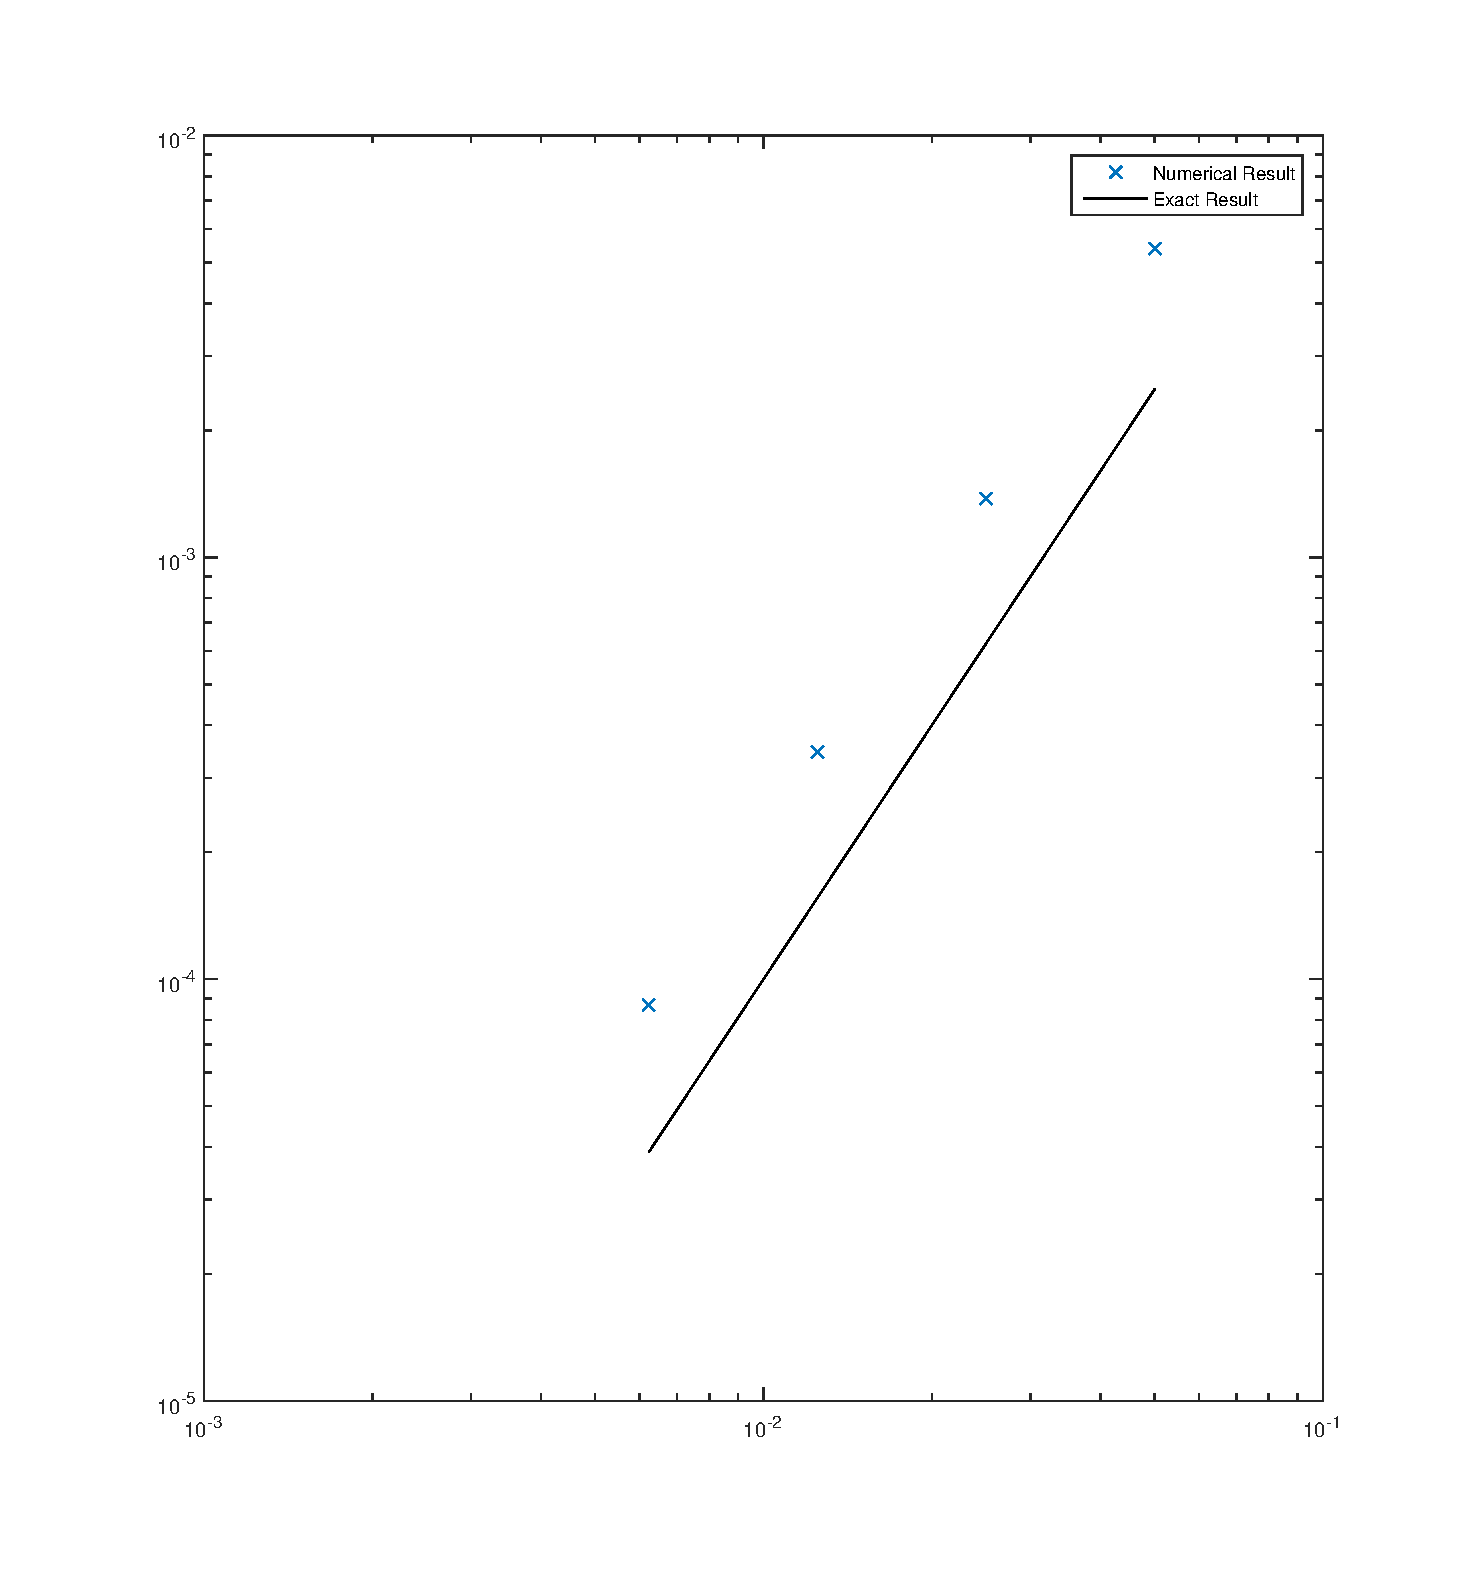
\includegraphics[width=3in]{nonConstConv}
\end{figure}


\eenum

\item Consider the wave equation
$$u_{tt}-u_{xx}=0,\;\;\;0<x<1,\;\;\;t>0$$
with initial conditions $u(x,0)=f(x), u_t(x,0)=0$ and boundary conditions $u(0,t)=u_x(1,t)=0.$
\benum
\item  Derive an exact solution to this system to use for verification.\\
Solution:\\
We begin by making the ansatz
$$u=\cos(\o t)\sin (kx)$$
which results in the relationship $\o=k$. We chose $\o=k=\pi/2$ so as to satisfy the boundary conditions. Thus the exact solution my code will be compared against is
$$u=\cos\left(\frac{\pi t}{2}\right)\sin\left(\frac{\pi x}{2}\right).$$

\item Convert this to a first-order system in space and time including the boundary and initial conditions.\\
Solution:\\
To convert the PDE into a first-order system, we let $v=u_t$ and $\sigma=u_x.$ Then we see $v_t=\sigma_x$ and $\sigma_t=v_x$, which we write in matrix form
$$\left[\begin{array}{c}v\\ \sigma\end{array}\right]_t=\left[\begin{array}{cc}0&1\\1&0\end{array}\right]\left[\begin{array}{c}v\\ \sigma\end{array}\right]_x.$$
The boundary conditions are transformed as follows.
$$u(0,t)=0\implies u_t(0,t)=0\implies v(0,t)=0.$$
$$u_x(1,t)=0=\sigma(1,t).$$
We can then use compatibility conditions to derive the boundary conditions for $v$ and $\sigma$ on the yet undetermined sides.
$$v(0,t)=0\implies v_t(0,t)=0=\sigma_x(0,t).$$
$$\sigma(1,t)=0\implies\sigma_t(1,t)=0=v_x(1,t).$$
Finally, the initial conditions are simply
$$u(x,0)=f(x)\implies u_x(x,0)=f'(x)=\sigma(x,0).$$
$$u_t(x,0)=0=v(x,0).$$


\item Using a collocated grid, write a centered spatially 2nd order accurate code, and use RK-4 as a time integrator. Verify that your code is 2nd order accurate using the solution derived in part(a).\\
Solution:\\
The centered spatially 2nd order accurate difference scheme takes the form
$$\left[\begin{array}{c}v_j\\ \sigma_j\end{array}\right]_t=\left[\begin{array}{cc}0&1\\1&0\end{array}\right]D_0\left[\begin{array}{c}v\\ \sigma\end{array}\right]=\frac{1}{2\Delta x}\left[\begin{array}{cc}0&1\\1&0\end{array}\right]\left[\begin{array}{c}v_{j+1}-v_{j-1} \\ \sigma_{j+1}-\sigma_{j-1}\end{array}\right].$$
Where $v_t$, $\sigma_t$ are integrated using RK-4. We now let $w=(v,\sigma)^T$, which allows us to rewrite the above formula nicely
$$w_{t,j}=\frac{1}{2\Delta x}A(w_{j+1}-w_{j-1}).$$
where 
$$A=\left[\begin{array}{cc}0&1\\1&0\end{array}\right].$$
For convenience, we refer to $g$ as follows:
$$g(w_j^n)=\frac{1}{2\Delta x}A(w_{j+1}^n-w_{j-1}^n).$$
Then, the time integration scheme looks like
$$w_j^{n+1}=w_j^n+\frac{\Delta t}{6}(k1_j^n+2k2_j^n+2k3_j^n+k4_j^n)$$
where 
$$k1_j^n=g(w_j^n),\;\;\; k2_j^n=g(w_j^n+\frac{dt}{2}k1_j^n),$$
$$k3_j^n=g(w_j^n+\frac{dt}{2}k2_j^n),\;\;\; k4_j^n=g(w_j^n+dt k3_j^n).$$
Note that $\Delta t=\nu \Delta x$ where $\nu$ is the cfl number, since the wave speed is given to be 1.\\
Initialization is trivial with this scheme, as we have an analytical expression for $w(x,0).$ given above. However, boundary conditions do require a bit of work. For the Nuemann conditions, we can simply use the even reflection that is characteristic there, i.e.,
$$\sigma_{-1}=\sigma_1,\;\;\; v_{N+1}=v_{N-1}.$$
For the Dirichlet conditions, we set $v_0=0$ and $\sigma_N=0.$ We can derive compatibility conditions here by differentiating twice in time and setting the resultant discretization to zero, for example,
$$v_{tt}(0,t)=v_{xx}(0,t)\approx D_+D_- v_0=0.$$
Applying this method to each boundary gives
$$v_{-1}=-v_1,\;\;\; \sigma_{N+1}=-\sigma_{N-1}.$$
A convergence test plot is presented here. We can see that the method is in fact 2nd order for both components. The code is presented at the end of this document.
\begin{figure}[h]
\centering
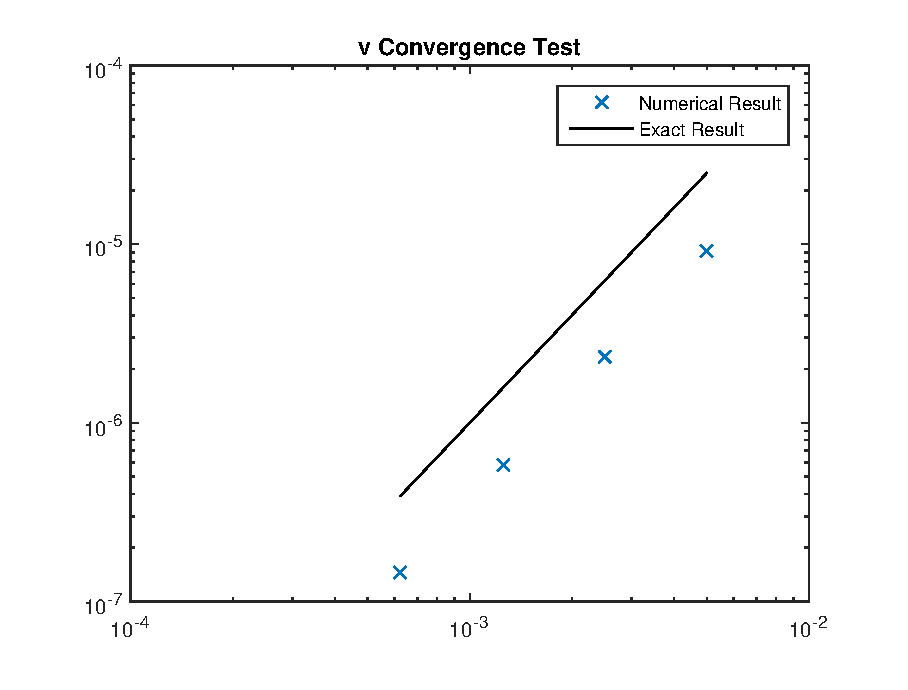
\includegraphics[width=3in]{colVConv}
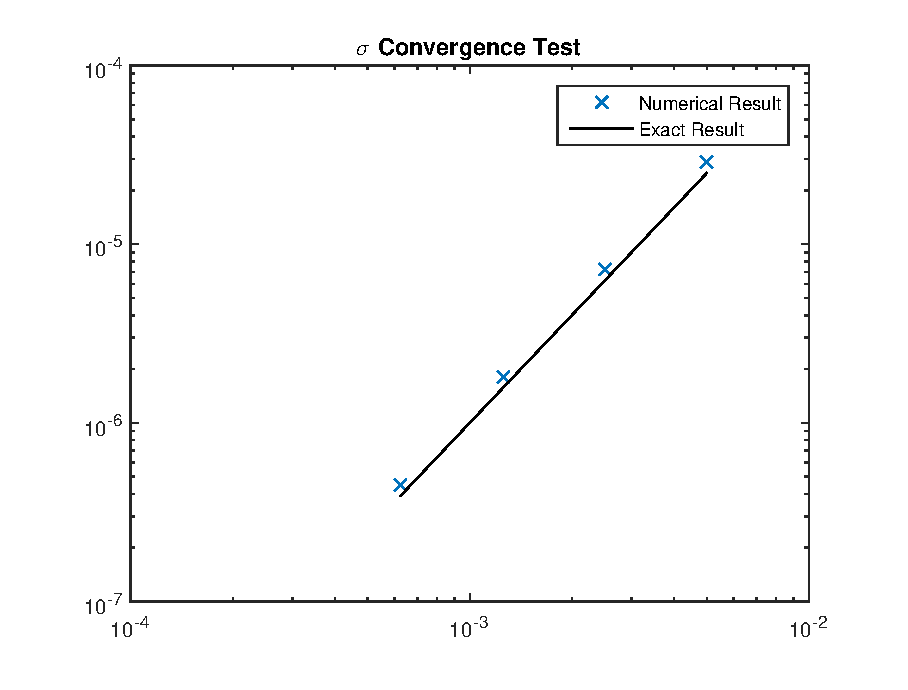
\includegraphics[width=3in]{colSConv}
\end{figure}

\item Run your code with the initial condition $f(x)=\exp(-100(x-.5)^2)$ and provide observations.\\
Solution:\\
The collocated grid solver has no problem with this initial data. The wave travels from inside out only to flip at the boundaries and return to the mirrored initial conditions. A plot of this is below. If ran for long enough time, the same behavior simply repeats itself. Note, this simulation, and the following two simulations were run with N=200.
\begin{figure}[h]
\centering
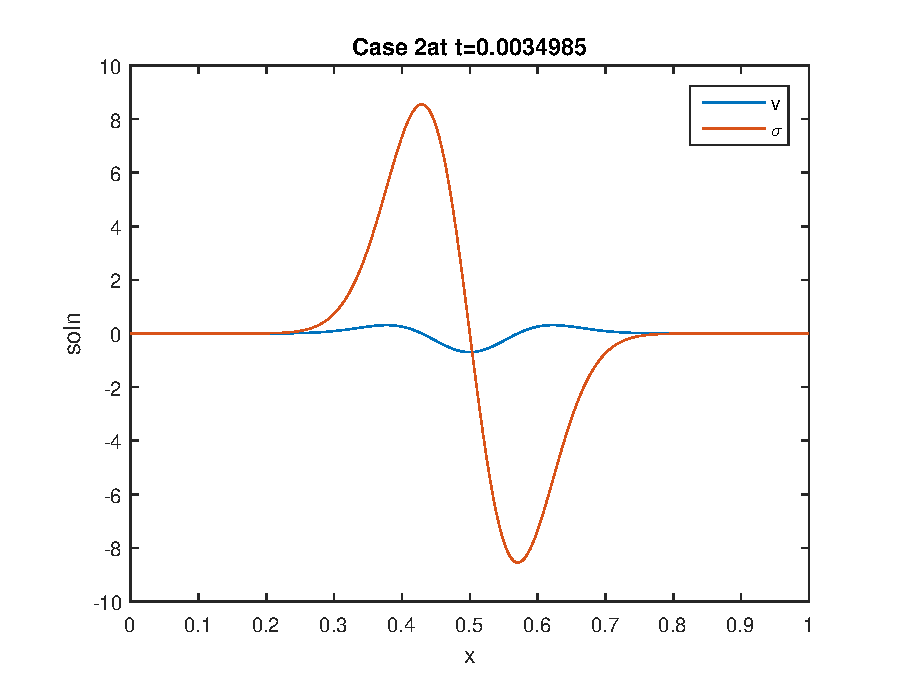
\includegraphics[width=3in]{initCol2}
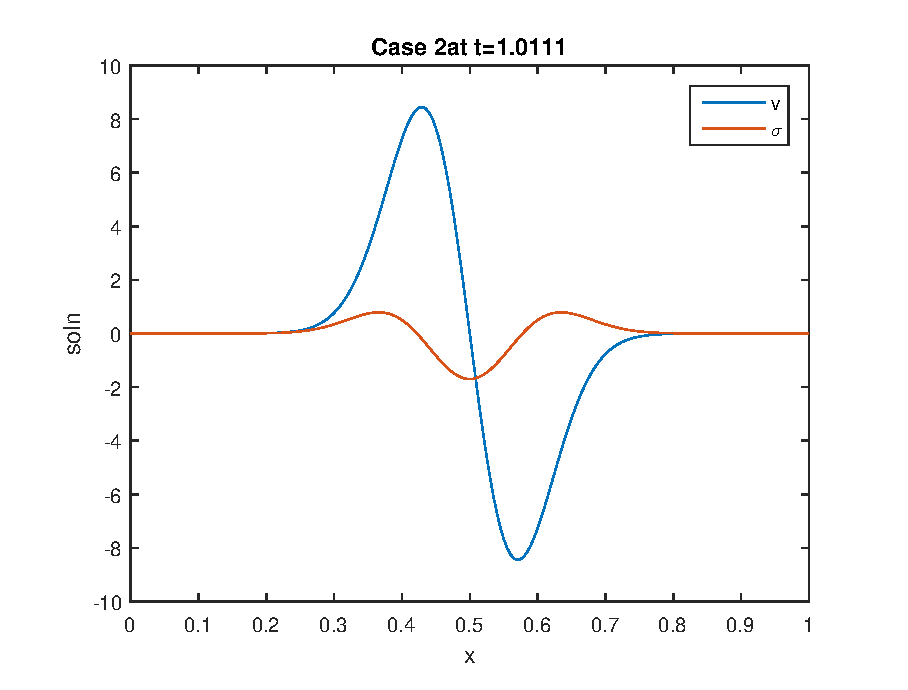
\includegraphics[width=3in]{endCol2}
\end{figure}
\item Run your code with the following initial condition and make observations about the results.
$$f(x)=\left\{\begin{array}{cc}4x-1&x\in(\frac{1}{4},\frac{1}{2}]\\-4x+3&x\in(\frac{1}{2},\frac{3}{4}]\\0&\text{ else }\end{array}\right.$$
Solution:\\
As the derivative needs to be passed into the code, we use the fourth order derivative discretization in space to find a discrete form of the derivative (in order to compare more effectively with the staggered grid code). The collocated grid solver seems to have some serious issues with this case, as the nonsmooth initial data rapidly devolves into rampant spiky oscillations. However, if run for appropriately long, the wave flips and returns to an approximation of the mirrored initial data much like the previous case, which is pictured below. This is sensible behavior because the initial conditions here can be viewed as a linearization of the initial conditions given in part d.

\begin{figure}[h]
\centering
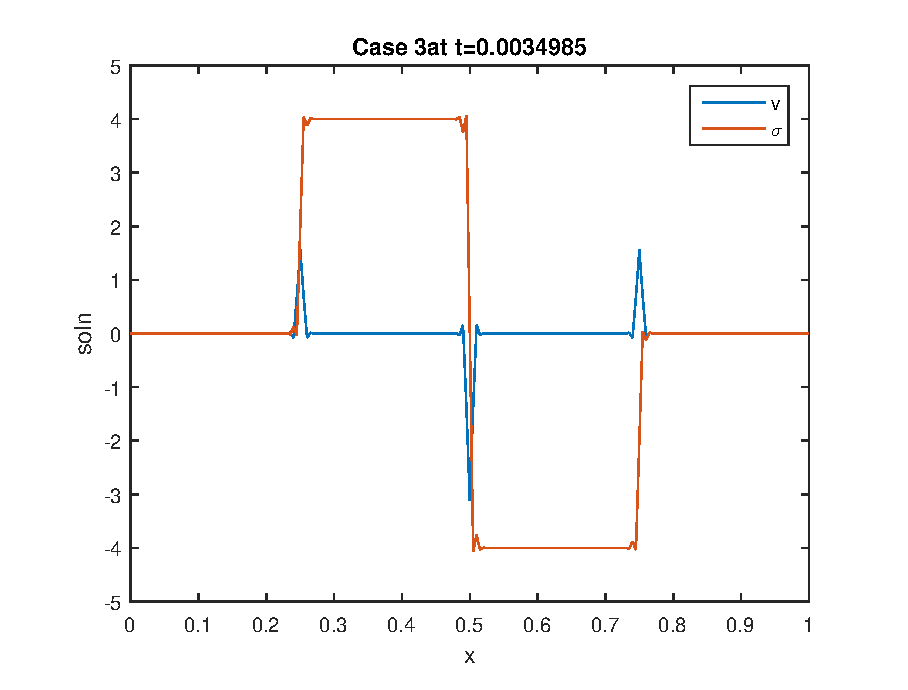
\includegraphics[width=3in]{initCol3}
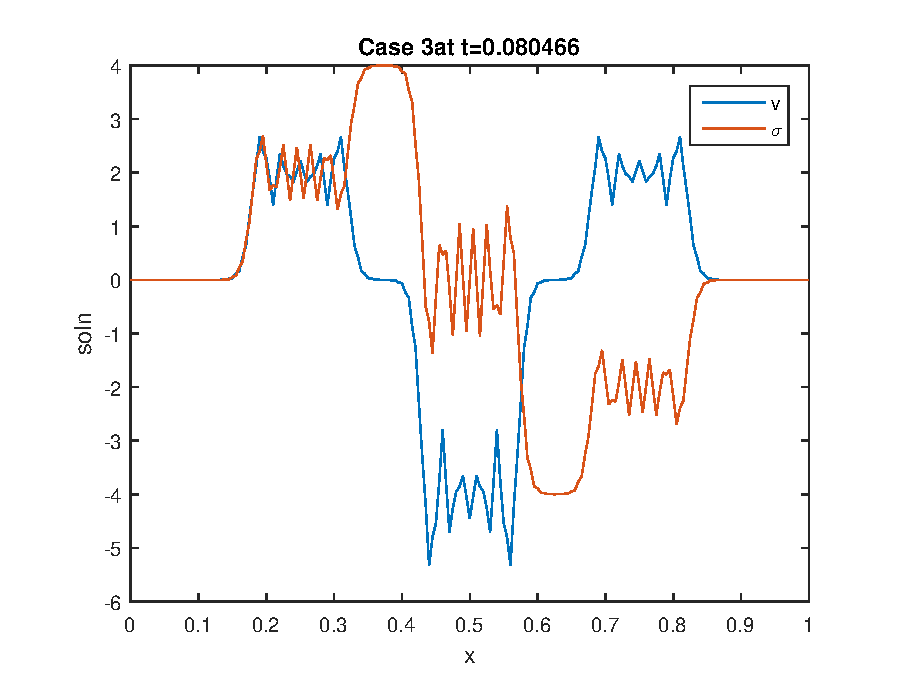
\includegraphics[width=3in]{midCol3}\\
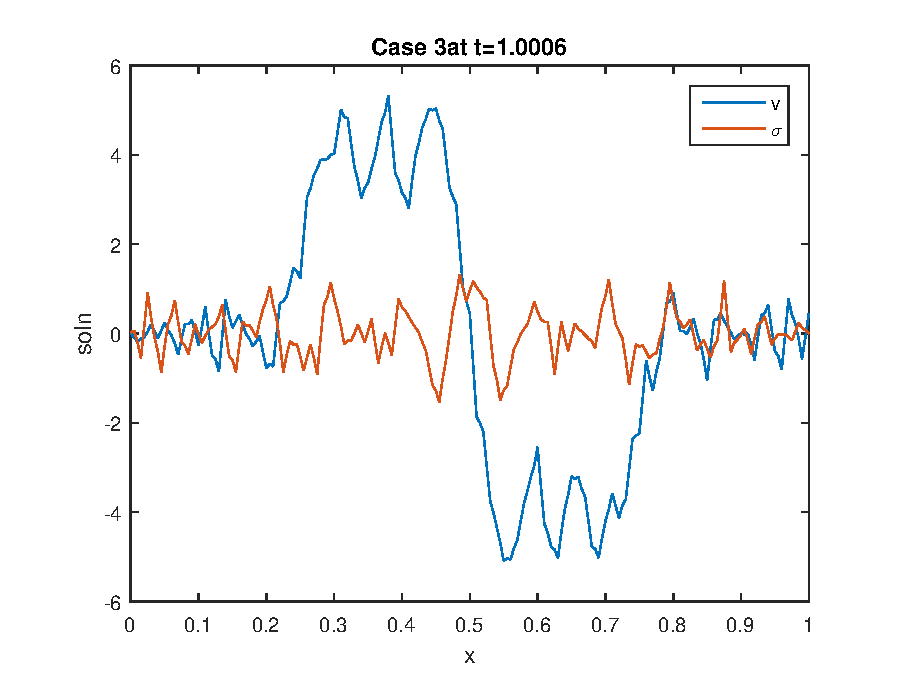
\includegraphics[width=3in]{endCol3}
\end{figure}
\item Run your code with the following initial condition and make observations about the results.
$$f(x)=\left\{\begin{array}{cc}1&x\in(\frac{1}{4},\frac{3}{4}\\ 0&\text{ else }\end{array}\right.$$
Solution:\\
Using the same setup as in the previous case, the collocated grid solver returns rapid oscillations that appear to be noise that becomes more obscure as time marches forward.
\begin{figure}[h]
\centering
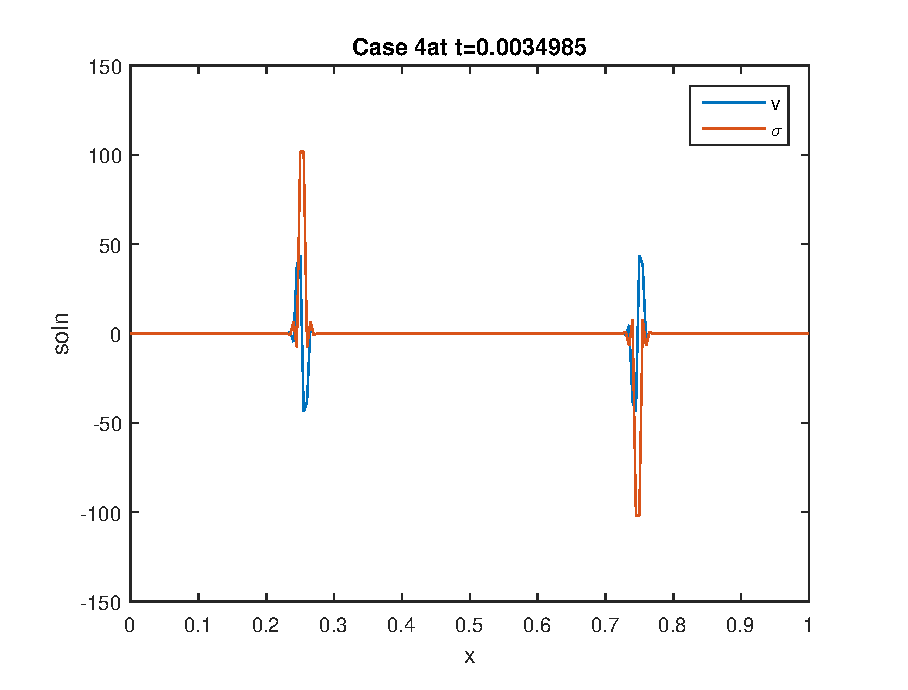
\includegraphics[width=3in]{initCol4}
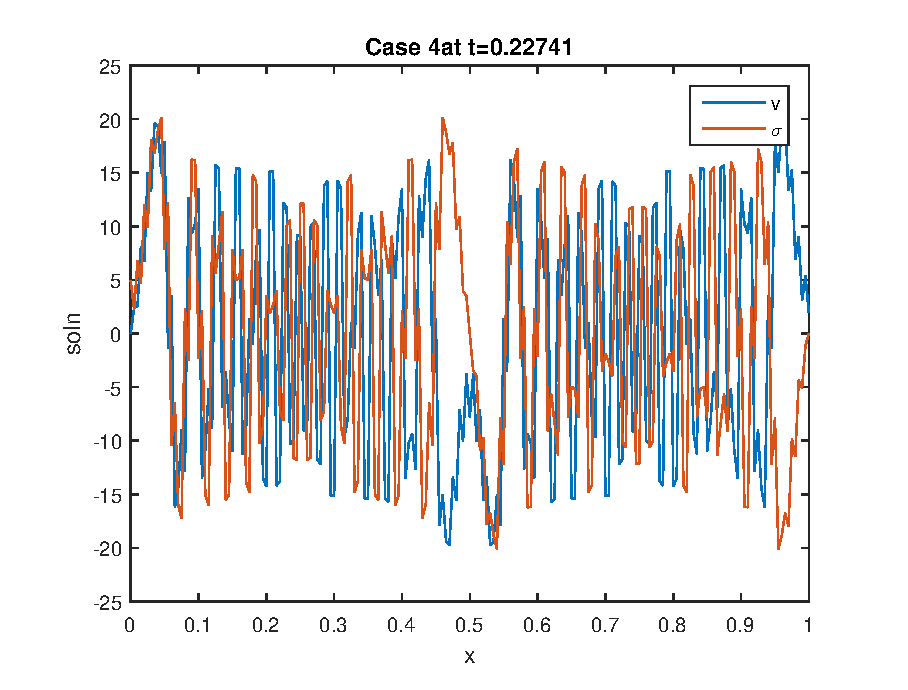
\includegraphics[width=3in]{midCol4}
\end{figure}
\begin{figure}[h]
\centering
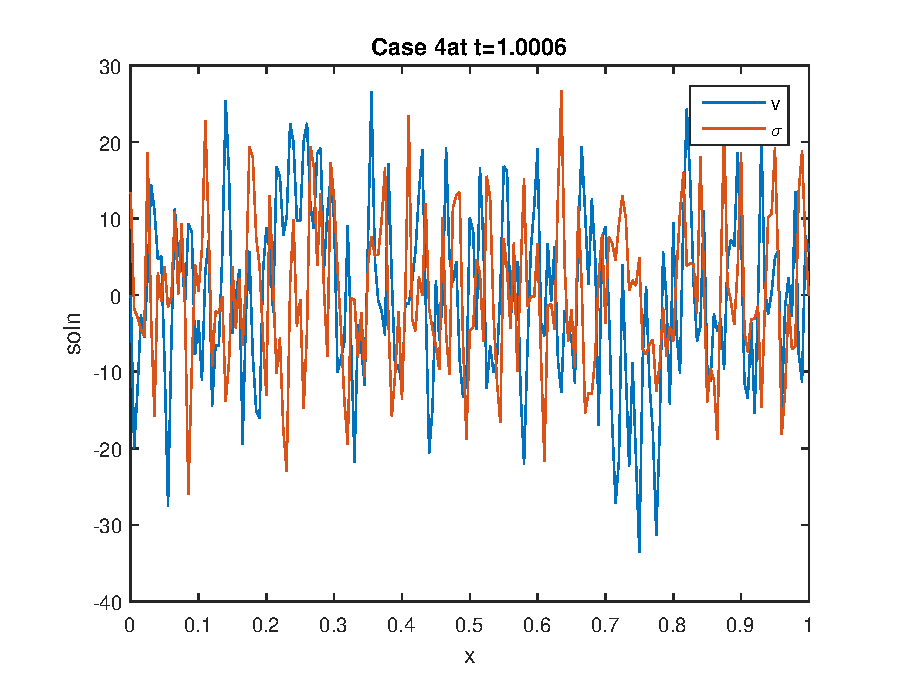
\includegraphics[width=3in]{endCol4}
\end{figure}
\eenum
\pagebreak
\item Repeat exercise 2, parts (c) through (f) above using a second order accurate staggered grid approach in space and time.\\ 
Solution:\\

We begin by defining two staggered grid spaces $x_L$ and $x_R$. The range of $x_L$ is from 0 to $1-dx/2,$ and the range of $x_R$ is from $dx/2$ to 1. We then define the grid points thus
$$x_{Li}=i\Delta x,\;\;\; x_{Ri}=(i+1/2)\Delta x.$$
Then we can set $v_i$ to live on $x_L$ and $\sigma_{i+1/2}$ to live on $x_{Ri}$. We note here that $\Delta x=1/(N-.5)$. The discretization we use is
$$v_i^{n+1}=v_i^n+\frac{\Delta t}{\Delta x}[\sigma_{i+1/2}^{n+1/2}-\sigma_{i-1/2}^{n+1/2}],$$
$$\sigma_{i+1/2}^{n+1/2}=\sigma_{i+1/2}^{n-1/2}+\frac{\Delta t}{\Delta x}[v_{i+1}^n-v_i^n].$$
The boundary conditions here are trivial, for we only loop over interior points, i.e., we do not loop over $x_{L0}=0$ or $x_{RN}=1,$ as we can use our Dirichlet conditions to ensure that these values for $v$ and $\sigma$ respectively are set to be 0. Initialization then is the last thing which needs to be discussed. For $v_i^n$ we can use the analytic condition discussed above. However, for $\sigma_{i+1/2}^{1/2}$ we must Taylor expand in time, which gives
$$\sigma_{i+1/2}^{1/2}=\sigma(x_{i+1/2},0)+\frac{\Delta t}{2}\sigma_t(x_{i+1/2},0)+\frac{\Delta t^2}{8}\sigma_{tt}(x_{i+1/2},0).$$
We simplify using the facts that $\sigma(x_{i+1/2},0)=f(x_{i+1/2}),$ $\sigma_t=v_x=0$ at $t=0$, and $\sigma_{tt}=\sigma_{xx}$, which results in the expression
$$\sigma_{i+1/2}^{1/2}=f'(x_{i+1/2})+\frac{dt^2}{8}f'''(x_{i+1/2}).$$
A convergence study plot is presented here. We can see that the code is 2nd order accurate. The code is attached at the end of this document. We can see from this that the convergence rate of the staggered code is slightly better than the convergence rate of the collocated code.
\begin{figure}[h]
\centering
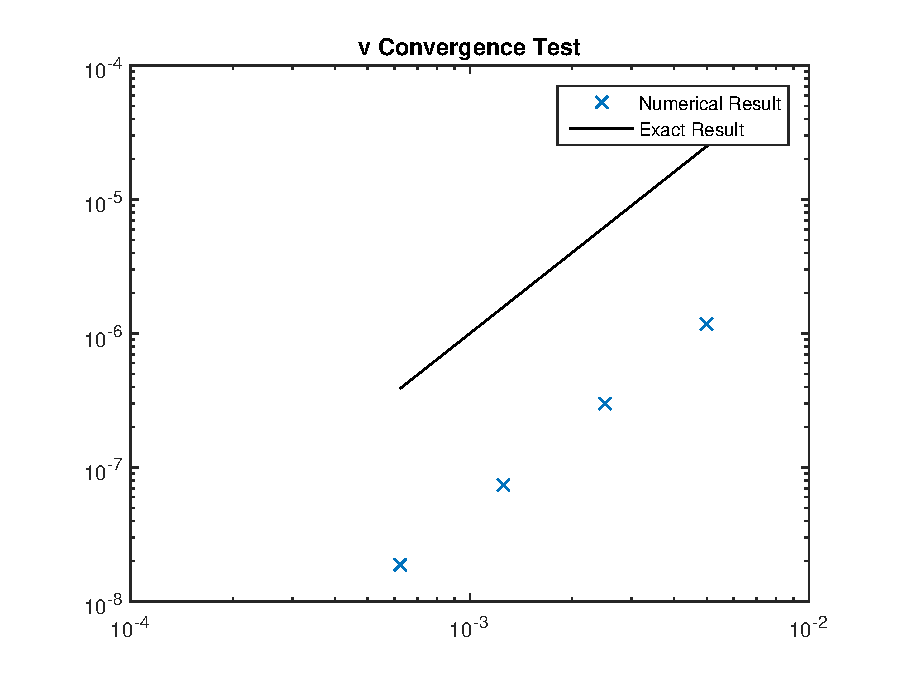
\includegraphics[width=3in]{stagVConv}
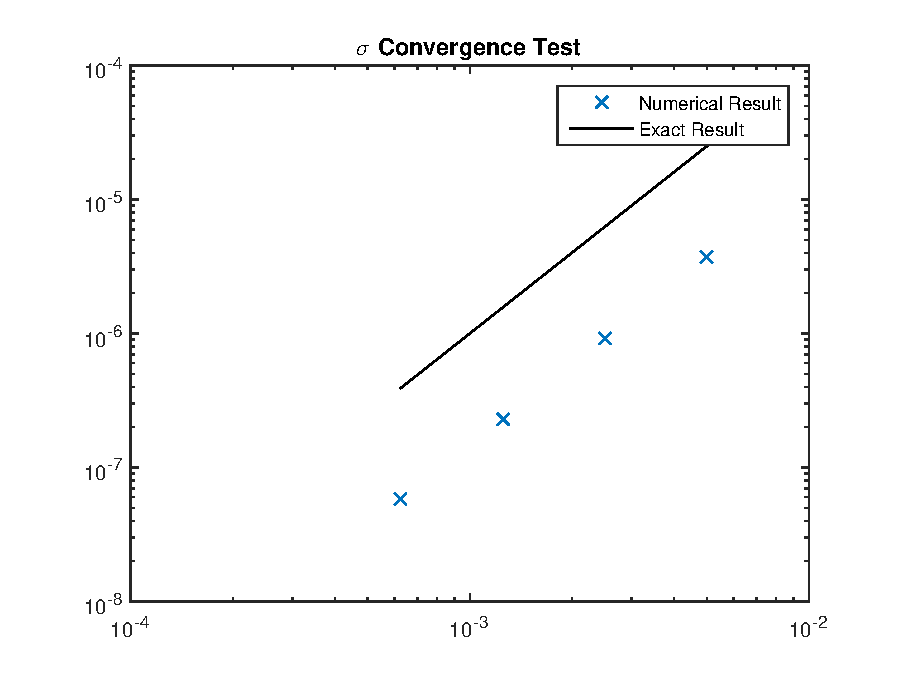
\includegraphics[width=3in]{stagSConv}
\end{figure}


We now run the initial conditions given in parts d,e,f of question 2.\\

(d) The staggered grid solver achieves about the same amount of smoothness and accuracy as the collocated grid solver when run with the Gaussian initial condition. A couple of plots are included below.
\begin{figure}[h]
\centering
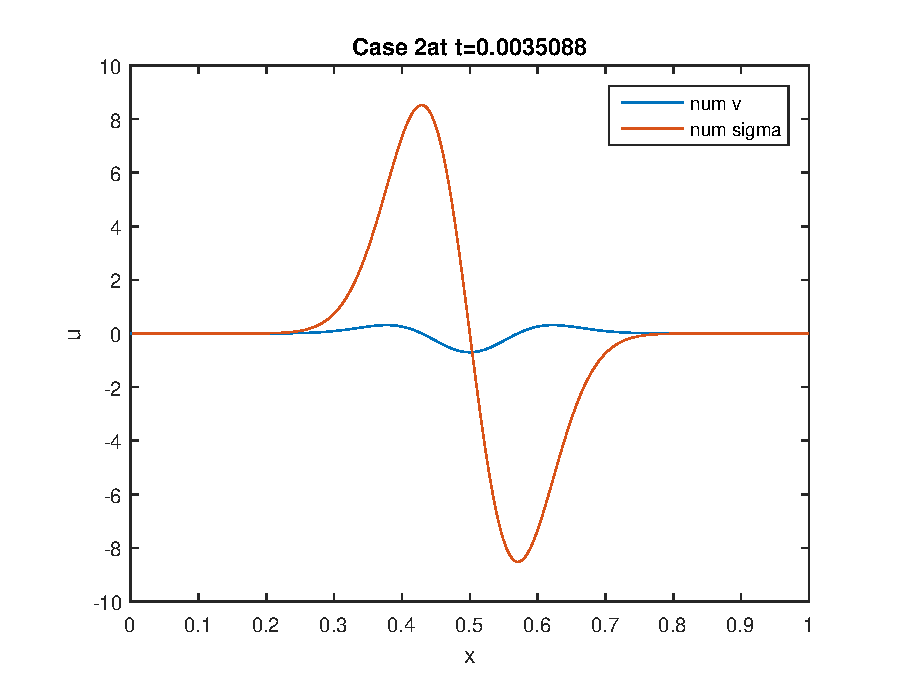
\includegraphics[width=3in]{initStag2}
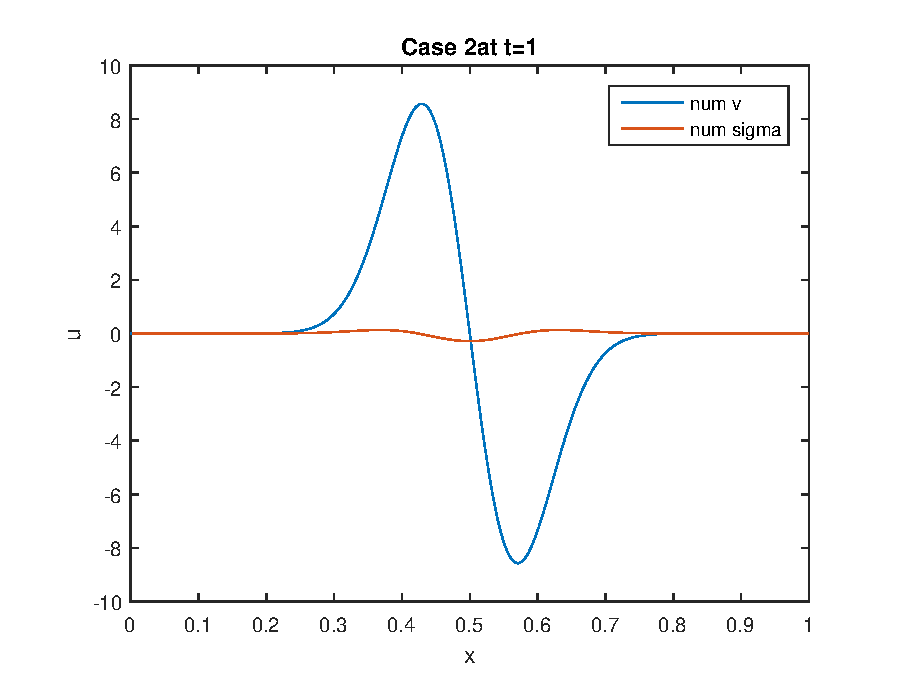
\includegraphics[width=3in]{endStag2}
\end{figure}

(e) Although far from perfect, the staggered grid solver performs considerably better given the nonsmooth initial data, as can be seen in the plots below. However, while oscillations are still present and unsightly, it is still clear what the solution is throughout out the run-time, and the oscillations are small and smooth.
\pagebreak
\begin{figure}[ht]
\centering
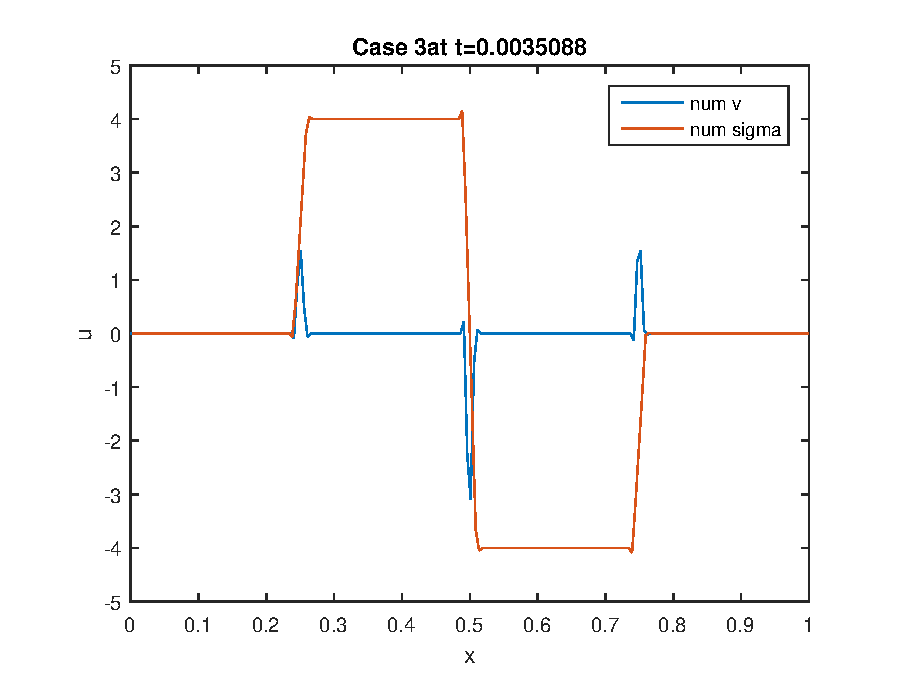
\includegraphics[width=3in]{initStag3}
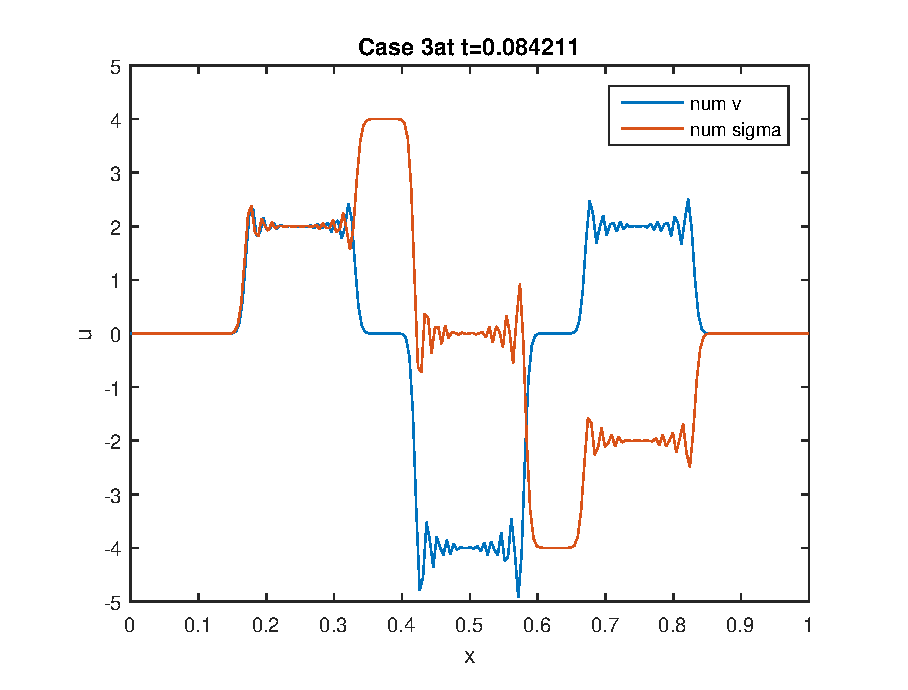
\includegraphics[width=3in]{midStag3}\\
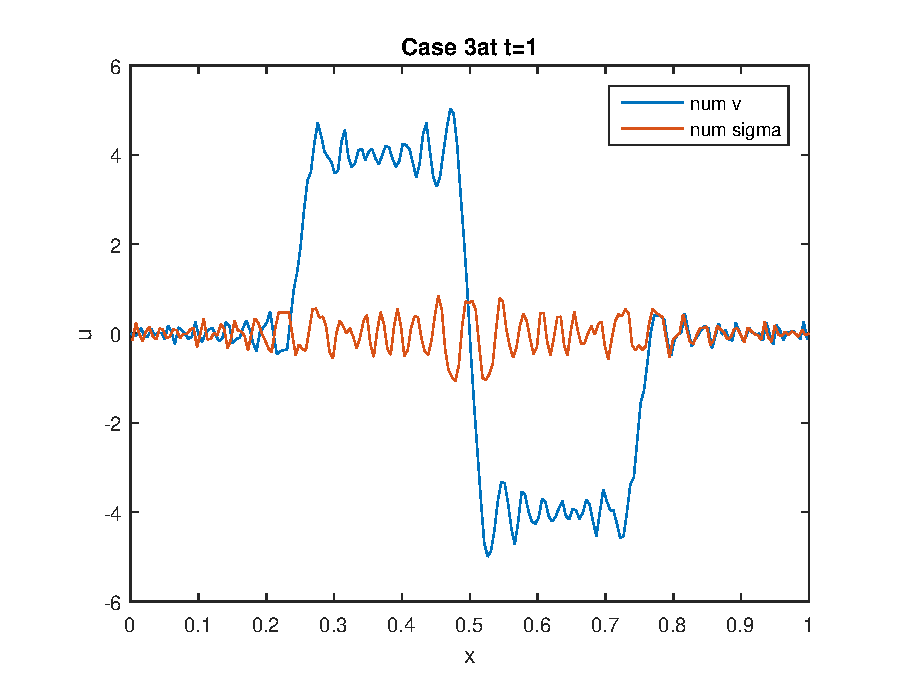
\includegraphics[width=3in]{endStag3}
\end{figure}

(f) For about $t<.4$ the staggered grid solver clearly outperforms the collocated grid solver. Oscillations are small and the solution can be easily determined from the graphs. However, if stepped much beyond that, the numerical solution appears to be little more than noise. 
\begin{figure}[b]
\centering
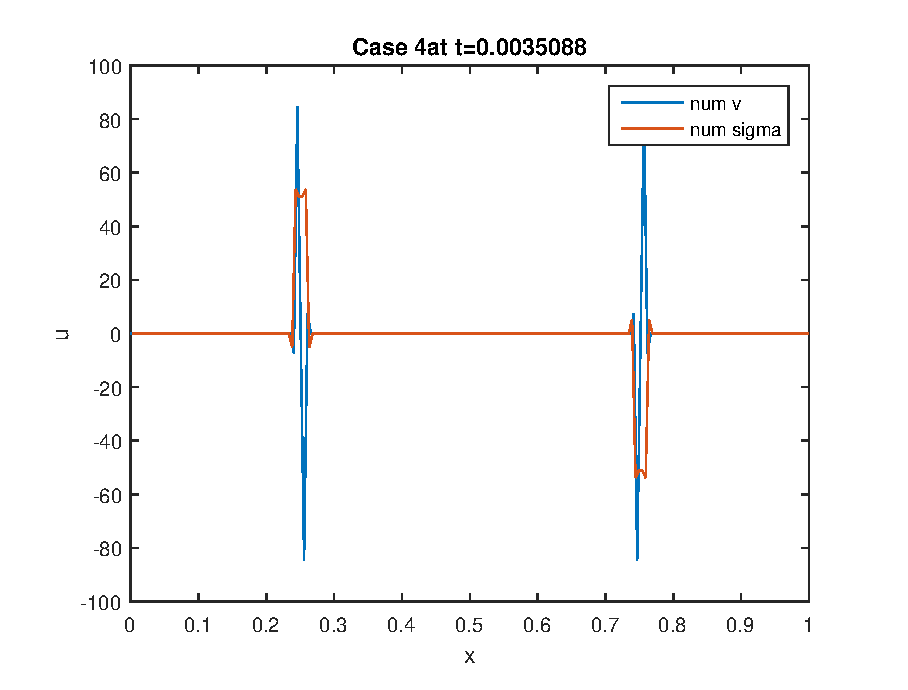
\includegraphics[width=3in]{initStag4}
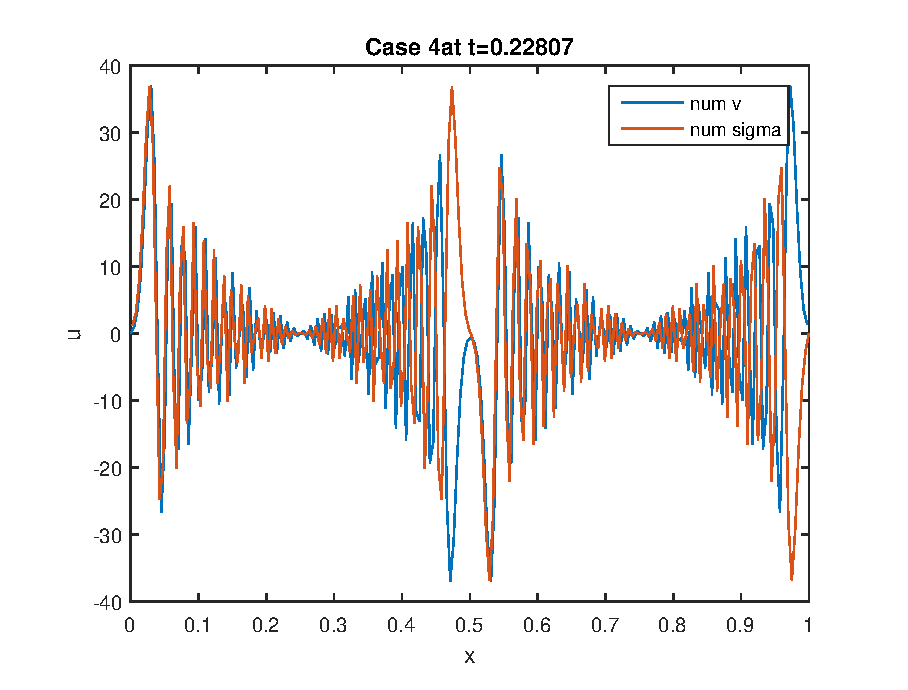
\includegraphics[width=3in]{midStag4}\\
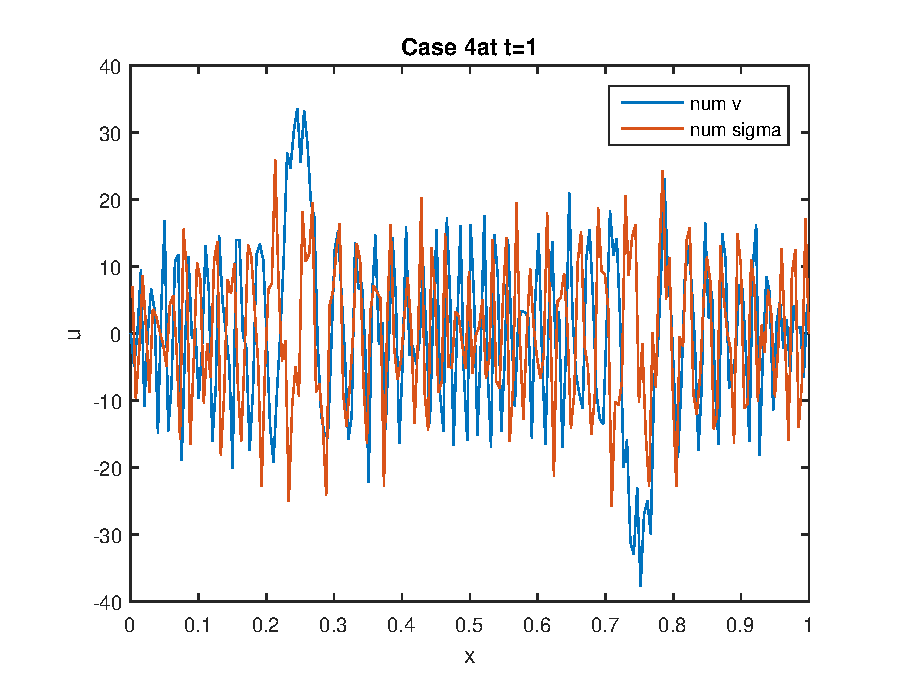
\includegraphics[width=3in]{endStag4}
\end{figure}
\eenum

\pagebreak

\bc {\bf Code Appendix} \ec
1. Nonconstant Coefficient Wave Equation Solver
\begin{lstlisting}[frame=single]
function [dx,err] = nonConstWave( N,xa,xb,tf,iPlot )
%xa=0;
%xb=1;

%% number of ghost points
ng = 1;
dx = (xb-xa)/N;
Ntot = N+2*ng;
%% first and last interior grid points
ia = ng+1;
ib = Ntot-ng;
x = linspace( xa+dx/2-ng*dx, xb-dx/2+ng*dx, Ntot );

%% grid size and other grid quantities

a=max(cos(x));
dt = 0.8*dx/a;
Nt = ceil( tf/dt );
dt = tf/Nt;


[unm1,un] = setICs( x,ia,ib,dx,dt);

%% allocate space for u
u = zeros(size(un));


%% Loop through time
t = dt;
for n = 1:Nt-1
    
    %% set BCs on un
    un = setBCs( un,ia,ib);
    
    %% compute update over domain interior
    for i = ia:ib
        i_plus=(i-1)*dx;
        i_minus=(i-2)*dx;
        uxx = ((c(i_plus))^2*(un(i+1)-un(i))-...
            (c(i_minus))^2*(un(i)-un(i-1)))/(dx^2);%+...
            %h(i_plus,t);
        u(i) = 2.*un(i)-unm1(i)+dt^2*(uxx+h(x(i),t));
    end   
        %% update solution histories
        unm1 = un;
        un   = u;
        t = t+dt;
        
        %% Plot Solution
        if( iPlot == 1 )
            plotStuff( x,u,ia,ib,t );
        end
       
    %% Check error
    u_exact = ue( x,t );
    
    ind = ia:ib;
    err = max(abs(u(ind)-u_exact(ind)));
%    return
end

%% Boundary condition setter
    function un = setBCs( un,ia,ib)
        un(ia-1)=un(ia);
        un(ib+1)=un(ib);
        return
    end

%% Exact Solution
    function z = ue( x,t )
        z = cos(t)*cos(pi*x);
        return
    end

    function z = uex ( x,t )
        z=-pi*cos(t)*sin(pi*x);
        return
    end

    function z= uett(x,t)
        z=-cos(t)*cos(pi*x);
        return
    end
    function z=uexx(x,t)
        z=-pi^2*cos(t)*cos(pi*x);
        return
    end
%% Source Term
    function z=h(x,t)
        z=uett(x,t)-2*c(x)*cx(x)*uex(x,t)-(c(x))^2*uexx(x,t);
        %z=(pi^2-1)*cos(pi*x)*cos(t);
        return
    end
%% Solution at t=0
    function z = f( x )
        z = cos(pi*x);
        return
    end
    function z = fp( x )
        z=-pi*sin(pi*x);
        return
    end

    function z=fpp( x )
        z=-pi^2*cos(pi*x);
        return
    end

    function z = g( x )
        % time derivative of solution at t=0
        z = 0;
        return
    end

%% Wave Speed
    function z=c(x)
        z=cos(x);
        %z=1;
        return
    end

    function z=cx(x)
        z=-sin(x);
        return
    end

%% Plot function
    function plotStuff( x,u,ia,ib,t )
        
        u_exact = ue( x,t );
        
        ind = ia:ib;
        subplot( 2,1,1 )
        plot( x(ind),u(ind),'rx', x(ind),u_exact(ind),'k-' );
        xlabel( 'x' );
        ylabel( 'u' );
        legend('Numerical Solution','Exact Solution')
        
        subplot(2,1,2)
        plot( x(ind),u(ind)-u_exact(ind),'rx' );
        xlabel( 'x' );
        ylabel( 'error' );
        drawnow;
        pause
        
        return
    end

%% Initial Condition setter
    function [unm1,un] = setICs( x,ia,ib,dx,dt )
        %% set intial condition at t=0 (and then BCs on initial condition)
        unm1 = zeros(size(x));
        for i = ia:ib
            unm1(i) = f( x(i) );
        end
        %plot(ia:ib,unm1)
        unm1 = setBCs(  unm1,ia,ib );
        
        %% now set initial condition at t=dt (and then BCs)
        %% here we use a Taylor expansion in time
        un = zeros(size(x));
        for i = ia:ib
            i_plus=(i-1)*dx;
            i_minus=(i-2)*dx;
            
            f0  = f(x(i));
            
            g0  = g(x(i));
            h0  = h(x(i),0);
            uxx = 2*c(x(i))*cx(x(i))*fp(x(i))+(c(x(i)))^2*fpp(x(i));
            %uxx = ((c(i_plus))^2*(unm1(i+1)-unm1(i))-...
            %(c(i_minus))^2*(unm1(i)-unm1(i-1)))/(dx^2);
            utt = uxx+h0;
            
            un(i) = f0+dt*g0+0.5*dt^2*(utt);
            
        end
        un = setBCs(  un,ia,ib);
        return
    end
end
\end{lstlisting}

2. Collocated FOS solver
\begin{lstlisting}[frame=single]
function [dx,v_err,sig_err]=colFOSsolver(N,xa,xb,cfl,tf,iPlot,Case)
% Solves the first order system for the wave equation on a collocated grid

%% Number of Ghost points
ng=1;
dx=(xb-xa)/N;
Ntot=N+1+2*ng;

%% first and last interior grid points
ia=ng+1;
ib=Ntot-ng;
x=linspace(xa-ng*dx,xb+ng*dx,Ntot);
x_ghost=linspace(xa-2*dx,xb+2*dx,Ntot+2);

%% grid size and other quantities

dt=cfl*dx;
Nt=ceil(tf/dt);
dt=tf/Nt;

[un]=setICs(x,x_ghost,dx,ia,ib,Case);

%% allocate space for u
u=zeros(size(un));

%% Loop through time
t=0;
for n=1:Nt-1
    %% Set BCs on u
    un=setBCs(un,ia,ib);
    %% Compute Runge-Kutta coefficient matrices
    [k1]=computeK(un,ia,ib,dx);
    [ua]=setBCs(un+dt*.5*k1,ia,ib);
    [k2]=computeK(ua,ia,ib,dx);
    [ub]=setBCs(un+dt*.5*k2,ia,ib);
    [k3]=computeK(ub,ia,ib,dx);
    [uc]=setBCs(un+dt*k3,ia,ib);
    [k4]=computeK(uc,ia,ib,dx);
    %% Compute update over domain interior
    for i=ia:ib
        u(:,i)=un(:,i)+dt/6*(k1(:,i)+2*k2(:,i)+2*k3(:,i)+k4(:,i));
    end

    %% update solution histories
    un=u;
    t=t+dt;
    
    %% Plot solution
    if(iPlot==1)
        plotStuff(x,u,ia,ib,t,Case);
    end
    
    %% Check error
    if Case==1
    [v,sigma]=ue(x,t);
    ind=ia:ib;
    v_err=max(abs(u(1,ind)-v(ind)));
    sig_err=max(abs(u(2,ind)-sigma(ind)));
    end
end

%% Compute k for RK4
    function K=computeK(un,ia,ib,dx)
        K=zeros(size(un));
        A=[0,1;1,0];
        for j=ia:ib
            K(:,j)=.5*A*(un(:,j+1)-un(:,j-1))/dx;
        end
        return
    end
%% Boundary condition setter
function un=setBCs(un,ia,ib)
    un(1,ia)=0;
    un(1,ia-1)=2*un(1,ia)-un(1,ia+1);
    un(2,ia-1)=un(2,ia+1);
    un(1,ib+1)=un(1,ib-1);
    un(2,ib)=0;
    un(2,ib+1)=2*un(2,ib)-un(2,ib-1);
    return
end

%% Exact Solution
    function [v,sigma]=ue(x,t)
        v=-pi*.5*sin(pi*t*.5)*sin(pi*x*.5);
        sigma=pi*.5*cos(pi*t*.5)*cos(pi*x*.5);
        
        return
    end

%% Solution at t=0
    function z=f(x,Case)
        if Case==1
            z=sin(pi*x*.5);
        elseif Case==2
            z=exp(-100*(x-.5)^2);
        elseif Case==3
            z=zeros(size(x));
            for m=1:numel(x)
                if x(m)>.25&&x(m)<=.5
                    z(m)=4*x(m)-1;
                elseif x(m)>.5&&x(m)<.75
                    z(m)=-4*x(m)+3;
                else
                    z(m)=0;
                end
            end
        elseif Case==4
            z=zeros(size(x));
            for m=1:numel(x)
                if x(m)>.25&&x(m)<.75
                    z=1;
                else
                    z=0;
                end
            end
        end
        return
    end

    function z=fx(m,x,dx,Case)
        if Case==1
            z=pi*.5*cos(pi*x(m)*.5);
        elseif Case==2
            z=-200*(x(m)-.5)*exp(-100*(x(m)-.5)^2);
        elseif Case==3 || Case==4
            % 4th order Dx of f(x)
            z=(-f(x(m+2),Case)+8*f(x(m+1),Case)-...
                8*f(x(m-1),Case)+f(x(m-2),Case))/(12*dx);
%         elseif Case==4
%             z=(f(x(m+1))-f(x(m-1)))/(2*dx);
        end
        return
    end

    function z=g(~)
        z=0;
        return
    end
%% Plot function
    function plotStuff( x,u,ia,ib,t,Case )
        if Case==1
        [v,sigma] = ue( x,t );
        
        ind = ia:ib;
        subplot( 2,1,1 )
        plot( x(ind),u(1,ind),'rx', x(ind),v(ind),'k-' );
        hold on
        plot(x(ind),u(2,ind),'bx',x(ind),sigma(ind),'g-');
        hold off
        xlabel( 'x' );
        ylabel( 'u' );
        legend('num v','exact v','num sigma','exact sigma')
        
        subplot(2,1,2)
        plot( x(ind),u(1,ind)-v(ind),'rx' );
        hold on
        plot(x(ind),u(2,ind)-sigma(ind),'bx');
        hold off
        xlabel( 'x' );
        ylabel( 'error' );
        drawnow;
        pause
        else
            ind=ia:ib;
            plot(x(ind),u(1,ind));
            hold on
            plot(x(ind),u(2,ind));
            hold off
            title(['Case ' num2str(Case) 'at t=' num2str(t)])
            %axis([0,1,-10,10])
            xlabel('x');
            ylabel('soln');
            legend('v','\sigma')
            drawnow
            pause
        end
        
        return
    end

%% Initial condition setter
    function [un]=setICs(x,x_ghost,dx,ia,ib,Case)
        %% set initial condition at t=0(then BCs on IC)
        un=zeros(2,numel(x));
        for j=ia:ib
            un(1,j)=0;
            un(2,j)=fx(j+1,x_ghost,dx,Case);
        end
        un=setBCs(un,ia,ib);
    end
end
\end{lstlisting}

3. Staggered FOS Solver
\begin{lstlisting}[frame=single]
function [dx,v_err,sig_err]=stagFOSsolver(N,xa,xb,cfl,tf,iPlot,Case)
% Solves the first order system for the wave equation on a staggered grid
%treat v=u_t and sigma=u_x separately
%% Number of Ghost points
ng=0;
dx=(xb-xa)/(N-.5);
Ntot=N+2*ng; %For each staggered grid

%% First and last interior grid points
% Staggered Left
ia=ng+1;
ib=Ntot-ng;
x_left=linspace(xa-ng*dx,xb-dx/2+ng*dx,Ntot);
%Staggered Right note ja=ia and jb=ib
ja=ng+1;
jb=Ntot-ng;
x_right=linspace(xa+dx/2-ng*dx,xb+ng*dx,Ntot);

%% Set up ghost grid for calculating fx and fxxx for the discontinuous cases
x_ghost=linspace(xa+dx/2-2*dx,xb+2*dx,N+4);
%% Grid size and other quantities
dt=cfl*dx;
Nt=ceil(tf/dt);
dt=tf/Nt;
[vn,sigman]=setICs(x_left,x_right,x_ghost,dx,dt,ja,jb,Case);
%% Allocate space for solution
v=zeros(1,Ntot);
sig=zeros(1,Ntot);
%% Loop through time
tv=0;
ts=dt/2;
for n=1:Nt-1
    %% Set BCs on sig and v
    [vn,sigman]=setBCs(vn,sigman,ia,jb);
    %% Compute update over domain interior

    for i=ia+1:ib
        v(i)=vn(i)+dt/dx*(sigman(i)-sigman(i-1));
    end
    for i=ja:jb-1
        sig(i)=sigman(i)+dt/dx*(v(i+1)-v(i));
    end
    
    %% Update solution histories
    sigman=sig;
    vn=v;
    tv=tv+dt;
    ts=ts+dt;
    
    %% Plot solution
    if iPlot==1
        plotStuff(x_left,v,x_right,sig,ia,ib,ja,jb,tv,ts,Case);
    end
    
    %% Check error
    if Case==1
    [ve,sige]=ue(x_left,x_right,tv,ts);
    ind=ia:ib;
    jnd=ja:jb;
    v_err=max(abs(v(ind)-ve(ind)));
    sig_err=max(abs(sig(jnd)-sige(jnd)));
    end
end

%% Boundary condition setter
    function [vn,sigman]=setBCs(vn,sigman,ia,jb)
        vn(ia)=0;
        sigman(jb)=0;
        return
    end
%% Initial condition setter
    function [vn,sigman]=setICs(x_left,x_right,x_ghost,dx,dt,ja,jb,Case)
        vn=zeros(1,numel(x_left));
        sigman=zeros(1,numel(x_right));
        for j=ja:jb-1
            sigman(j)=fx(j+2,x_ghost,dx,Case)+dt^2/8*fxxx(j+2,x_ghost,dx,Case);
        end
        [vn,sigman]=setBCs(vn,sigman,1,jb);
        return
    end
        
%% Exact Solution
    function [ve,sige]=ue(x_left,x_right,tv,ts)
        
        ve=-pi*.5*sin(pi*tv*.5)*sin(pi*x_left*.5);
        sige=pi*.5*cos(pi*ts*.5)*cos(pi*x_right*.5);
        return
    end

%% Solution at t=0
    function z=f(x,Case)
        %z=sin(pi*x*.5);
        if Case==1
            z=sin(pi*x*.5);
        elseif Case==2
            z=exp(-100*(x-.5)^2);
        elseif Case==3
            z=zeros(size(x));
            for m=1:numel(x)
                if x(m)>.25&&x(m)<=.5
                    z(m)=4*x(m)-1;
                elseif x(m)>.5&&x(m)<.75
                    z(m)=-4*x(m)+3;
                else
                    z(m)=0;
                end
            end
        elseif Case==4
            z=zeros(size(x));
            for m=1:numel(x)
                if x(m)>.25&&x(m)<.75
                    z=1;
                else
                    z=0;
                end
            end
        end
        return
    end
%     function z=fx(x)
%         z=pi*.5*cos(pi*x*.5);
%         return
%     end
    function z=fx(m,x,dx,Case)
        if Case==1
            z=pi*.5*cos(pi*x(m)*.5);
        elseif Case==2
            z=-200*(x(m)-.5)*exp(-100*(x(m)-.5)^2);
        elseif Case==3 || Case==4
            % 4th order Dx of f(x)
            z=(-f(x(m+2),Case)+8*f(x(m+1),Case)-...
                8*f(x(m-1),Case)+f(x(m-2),Case))/(12*dx);
%         elseif Case==4
%             z=(f(x(m+1))-f(x(m-1)))/(2*dx);
        end
        return
    end
    function z=fxxx(m,x,dx,Case)
        if Case==1
            z=-(pi*.5)^3*cos(pi*x(m)*.5);
        else
            %2nd order Dxxx of f
            z=(f(x(m+2),Case)-2*f(x(m+1),Case)+2*f(x(m-1),Case)-...
                f(x(m-2),Case))/(2*dx^3);
        end
        return
    end
%% Plot function
    function plotStuff(x_left,v,x_right,sig,ia,ib,ja,jb,tv,ts,Case)
        if Case==1
        [ve,sige]=ue(x_left,x_right,tv,ts);
        ind=ia:ib;
        jnd=ja:jb;
        subplot(2,1,1)
        plot(x_left(ind),v(ind),'rx',x_left(ind),ve(ind),'k-');
        hold on
        plot(x_right(jnd),sig(jnd),'bx',x_right(jnd),sige(jnd),'g-');
        hold off
        xlabel('x')
        ylabel('u')
        legend('num v', 'exact v', 'num sig','exact sig')
        
        subplot(2,1,2)
        plot(x_left(ind),v(ind)-ve(ind),'rx')
        hold on
        plot(x_right(jnd),sig(jnd)-sige(jnd),'bx')
        hold off
        xlabel('x')
        ylabel('error')
        drawnow;
        pause
        else
            ind=ia:ib;
            plot(x_left(ind),v(ind));
            hold on
            plot(x_right(ind),sig(ind));
            hold off
            xlabel('x')
            ylabel('u')
            legend('num v','num sigma')
            title(['Case ' num2str(Case) 'at t=' num2str(tv)])
            drawnow
            pause
        end
    end
end
\end{lstlisting}
\end{document}
